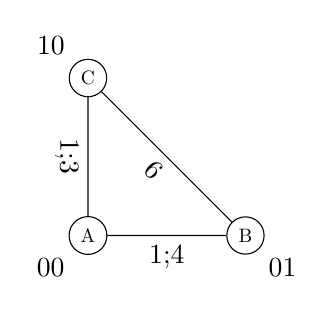
\begin{tikzpicture}[gv/.style={draw=black,circle,scale=0.7},scale=2]
\node[gv] (A) at (0,0) {A}; \draw (A.south west) node[anchor=north east] {$00$};
\node[gv] (B) at (1,0) {B}; \draw (B.south east) node[anchor=north west] {$01$};
\node[gv] (C) at (0,1) {C}; \draw (C.north west) node[anchor=south east] {$10$};
\draw (A) to node[sloped,below] {1;4} (B) to node[sloped,below] {6} (C) to node[sloped,below] {1;3} (A);
\end{tikzpicture}